%Appendix
\begin{figure}[h!]
	
	%\centering centers the figure on the page.  This is convention.

	\vspace{-4.7em}
	\centerline{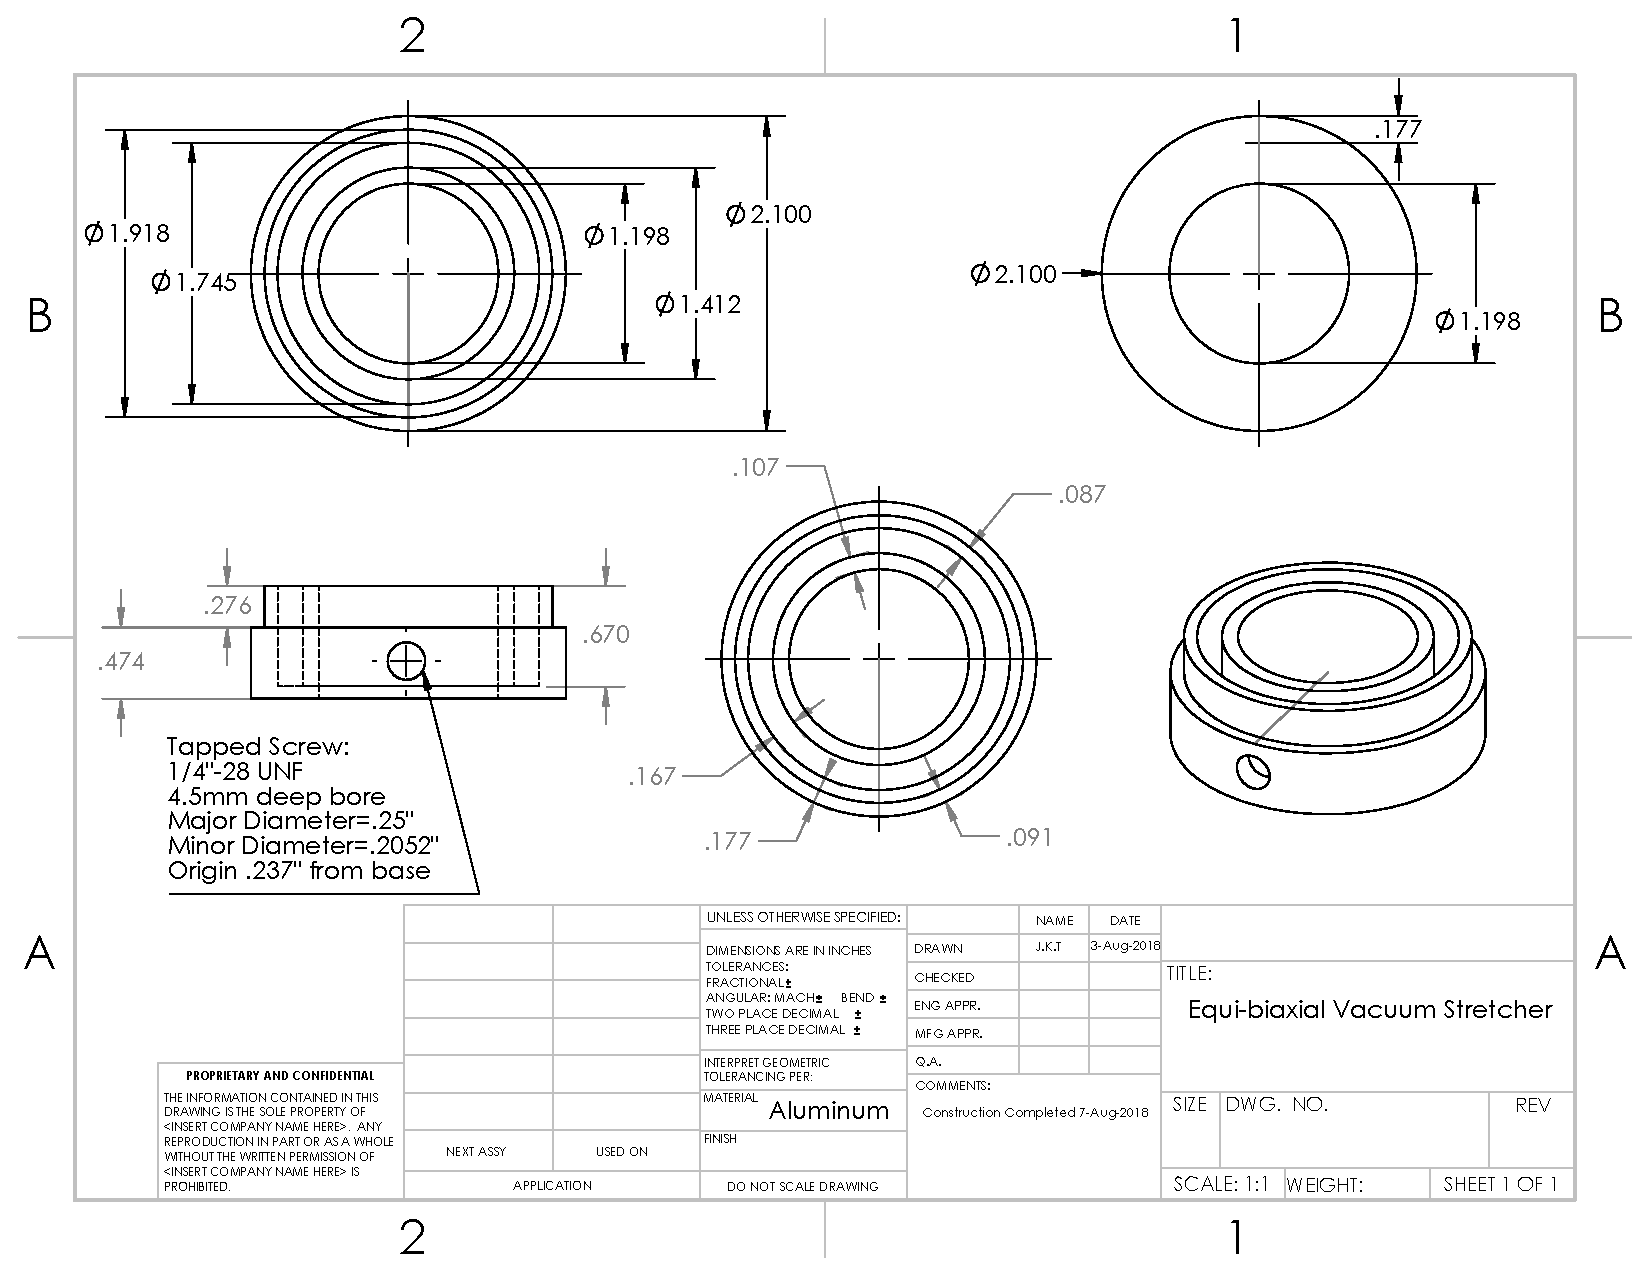
\includegraphics[scale=.65]{Chapters/Figures/Stretcher_body_with_screwtap_updated.PDF}}
	 
	\caption[Stretching Apparatus Design Document]{The equi-biaxial vacuum stretcher design document. Note: all measurements are in inches.}
	
%	This reference can be called in the text using the \ref tag.
	\label{fig:stretcherDesignBase}
\end{figure}


\begin{figure}[h!]
	%\centering centers the figure on the page.  This is convention.
	
	
	\centerline{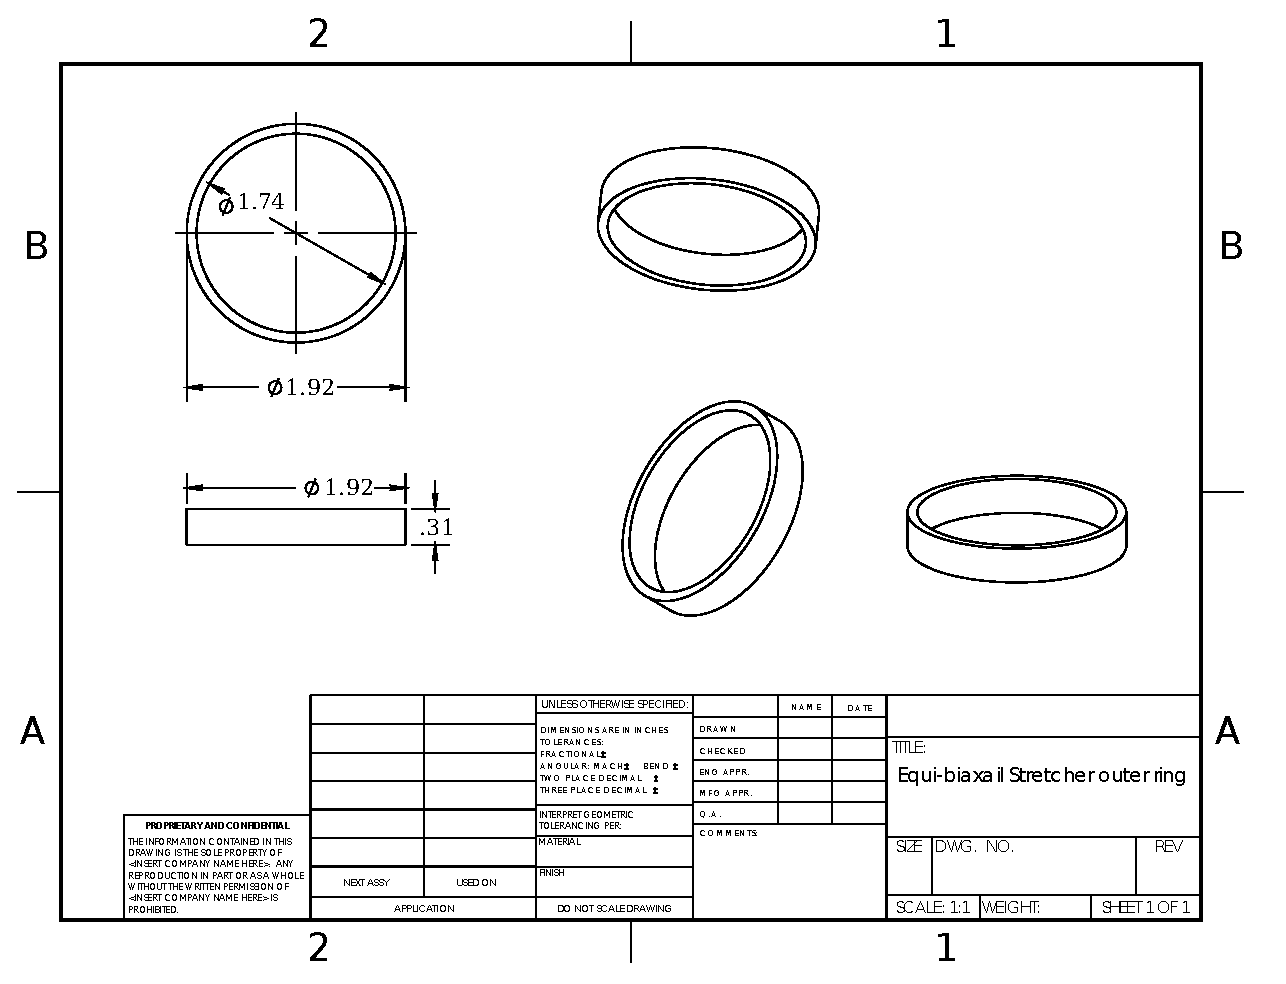
\includegraphics[scale=.85]{Chapters/Figures/Stretcher_outer.pdf}}
	\vspace{-.7em}
	\caption[Stretcher outer-ring]{Engineering Design Document of the outer-ring for the Stretching Apparatus. Note: all measurements are in millimeters. (UGH, why is the base in imperial and the ring in metric?! Must fix this - Jeremy )}
	
	%	This reference can be called in the text using the \ref tag.
	\label{fig:stretcherDesignRing}
\end{figure}

%Appendices are a good idea for almost any thesis.  Your main thesis body will likely contain perhaps 40-60 pages of text and figures.  You may well write a larger document than this, but chances are that some of the information contained therein, while important, does \emph{not} merit a place in the main body of the document.  This sort of content - peripheral clarifying details, computer code, information of use to future students but not critical to understanding your work \ldots - should be allocated to one or several appendices.  
